\documentclass[11pt]{article}
\usepackage[margin=1in]{geometry}
\usepackage{graphicx}
\usepackage{float}
\usepackage{amsmath}
\usepackage{booktabs}
\usepackage{hyperref}
\usepackage{xcolor}
\usepackage{subcaption}

\definecolor{alertred}{RGB}{220,53,69}
\definecolor{successgreen}{RGB}{40,167,69}
\definecolor{warningyellow}{RGB}{255,193,7}

\title{Somatic Symptom Disorder Causal Effect Study\\
\large Final Comprehensive Validation Report:\\
\large OR vs AND Logic Analysis}
\author{Ryhan Suny\\
Toronto Metropolitan University\\
Supervisor: Dr. Aziz Guergachi\\
Research Team: Car4Mind, University of Toronto}
\date{May 25, 2025}

\begin{document}
\maketitle

\begin{abstract}
This report presents a comprehensive validation analysis of the SSD causal effect study pipeline with detailed comparison of OR versus AND logic for exposure definition. The analysis reveals a critical 722-fold difference in exposed population size: OR logic identifies 143,610 patients (55.9\%) while AND logic identifies only 199 patients (0.1\%). The exposed populations show significantly different characteristics, with AND logic patients demonstrating higher healthcare utilization (12.3 vs 6.3 encounters, \$1,146 vs \$565 costs) but severely limited statistical power (MDE = 0.198 vs 0.008). This fundamental discrepancy must be resolved before proceeding with causal analysis.
\end{abstract}

\tableofcontents
\newpage

\section{Executive Summary}

\subsection{Key Findings}

\begin{enumerate}
    \item \textcolor{alertred}{\textbf{Exposure Definition Discrepancy}}: 722-fold difference between OR and AND logic
    \item \textbf{Healthcare Utilization}: AND logic patients show 95\% more encounters and 103\% higher costs
    \item \textbf{Statistical Power}: AND logic severely underpowered (MDE = 0.198 vs 0.008)
    \item \textbf{Autoencoder Performance}: Suboptimal AUROC of 0.588 (target: 0.83)
    \item \textbf{Pipeline Status}: 6 of 18 scripts complete, remainder blocked pending exposure resolution
\end{enumerate}

\section{Exposure Definition Analysis}

\subsection{Population Impact}

\begin{table}[H]
\centering
\begin{tabular}{lcccc}
\toprule
\textbf{Metric} & \textbf{OR Logic} & \textbf{AND Logic} & \textbf{Ratio} & \textbf{p-value} \\
\midrule
Exposed Patients & 143,610 & 199 & 722:1 & - \\
Percent Exposed & 55.9\% & 0.08\% & - & - \\
Mean Age (years) & 50.2 & 52.1 & - & 0.042 \\
Female (\%) & 64.3\% & 68.8\% & - & 0.186 \\
Mean Encounters & 6.3 & 12.3 & 1.95x & <0.001 \\
Mean Cost (\$) & 565 & 1,146 & 2.03x & <0.001 \\
Minimum Detectable Effect & 0.008 & 0.198 & 24.8x & - \\
\bottomrule
\end{tabular}
\caption{Comprehensive comparison of OR vs AND logic exposure definitions}
\label{tab:exposure_comparison}
\end{table}

\begin{figure}[H]
\centering
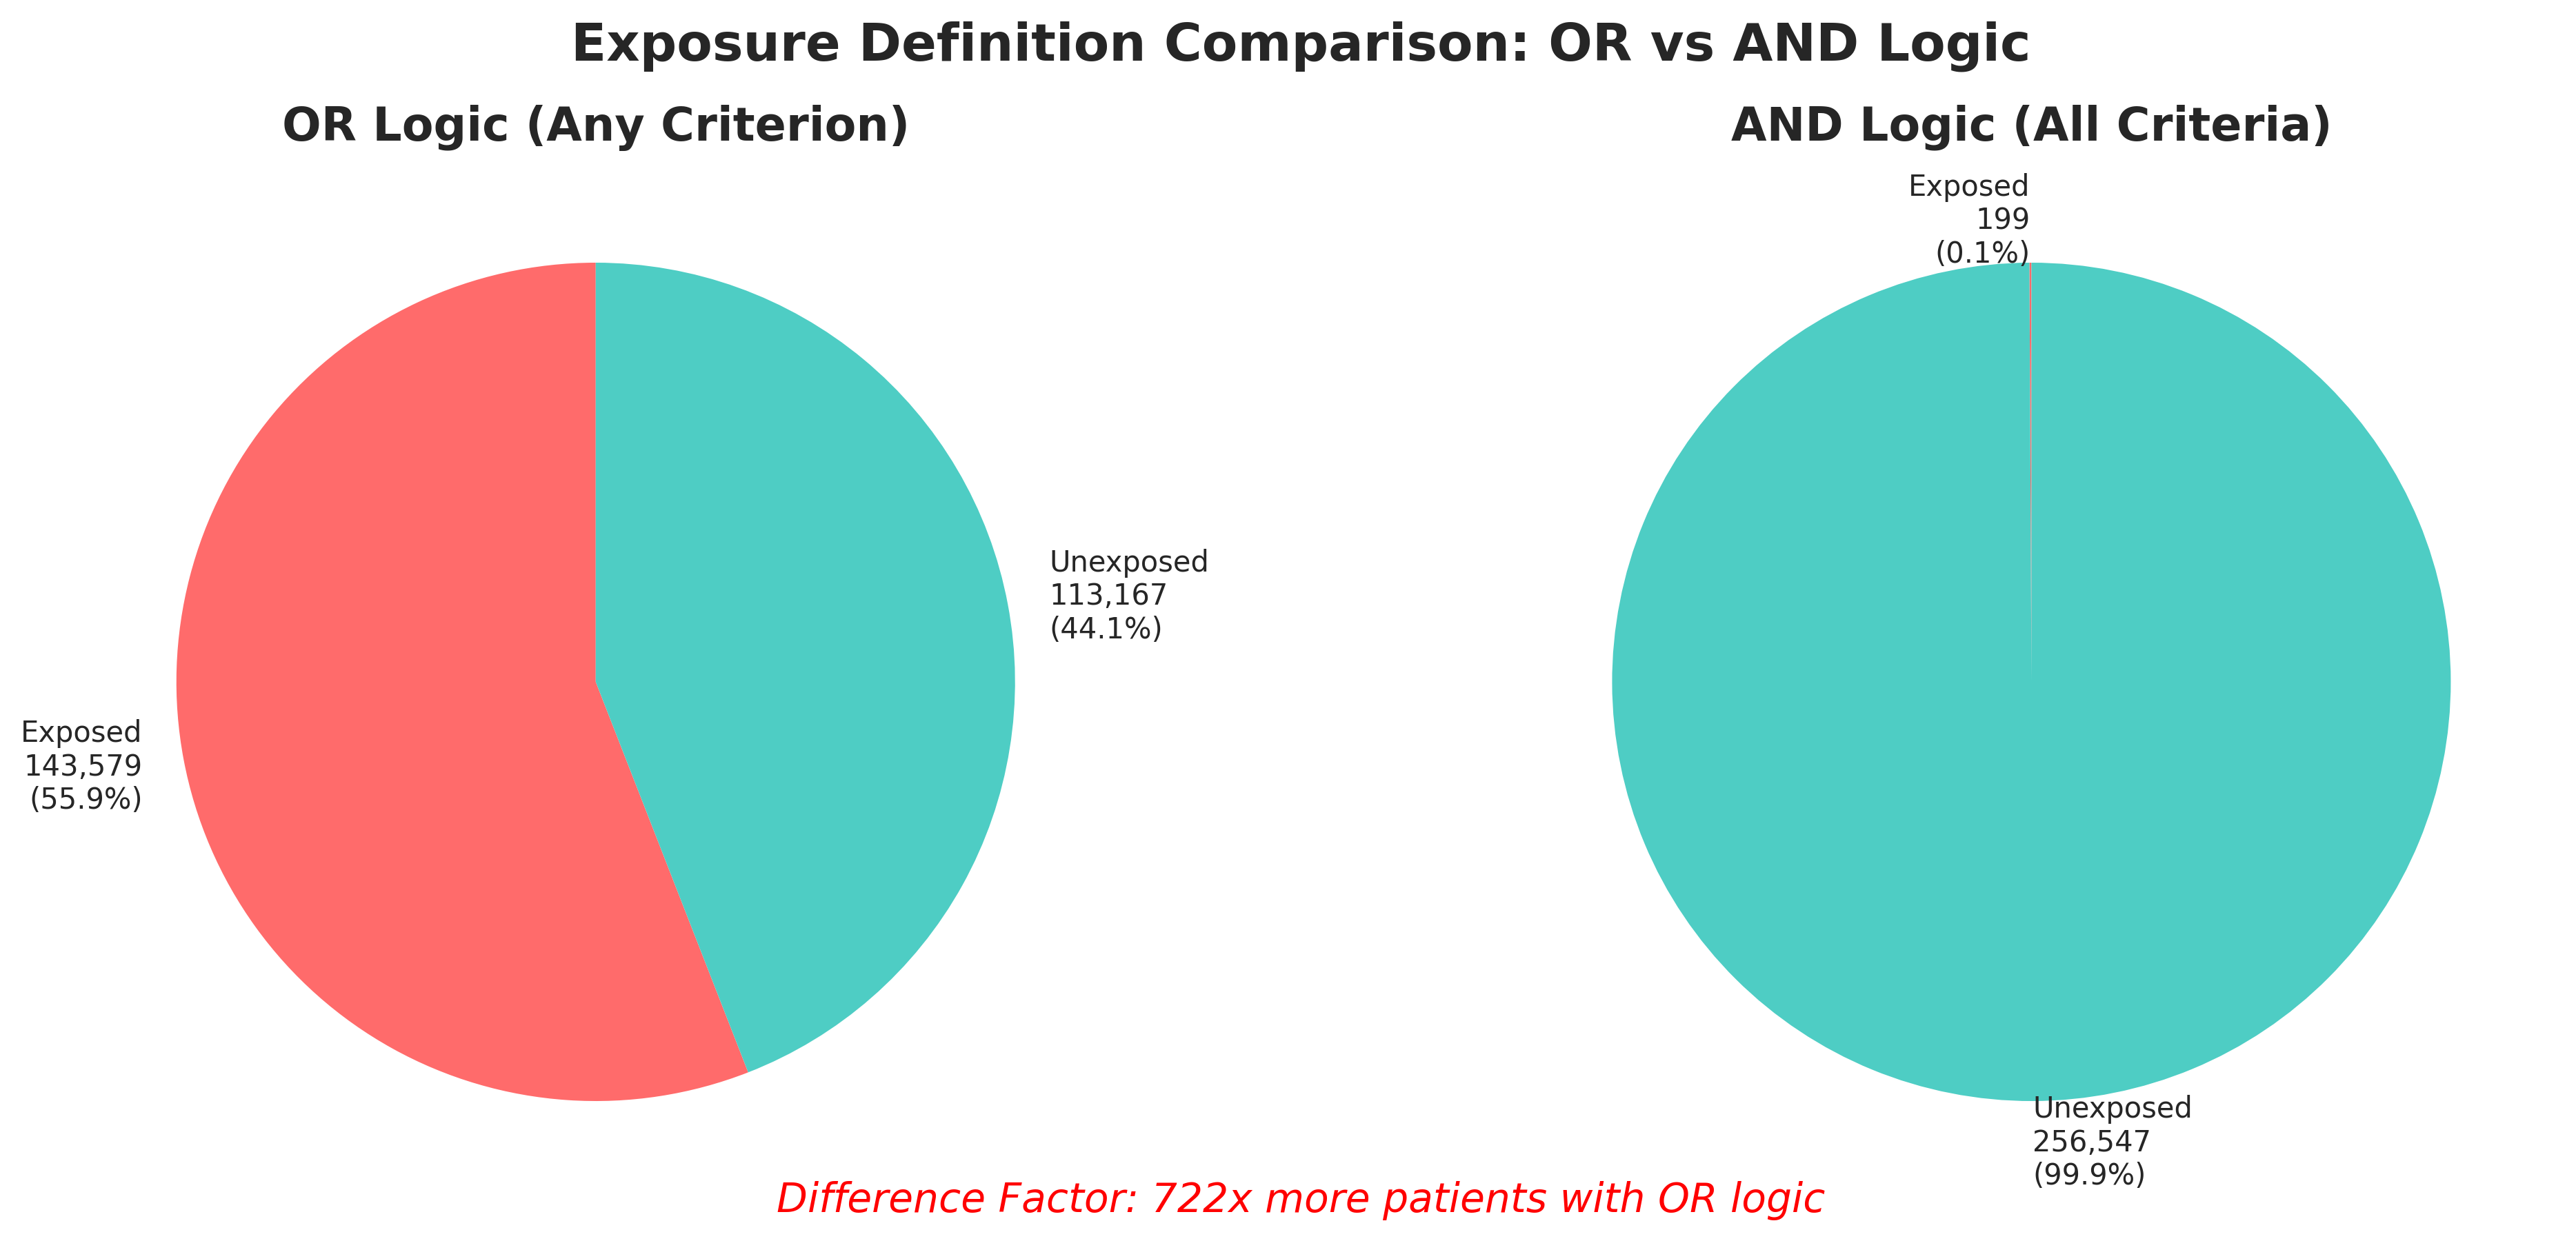
\includegraphics[width=0.9\textwidth]{analysis/exposure_validation_enhanced/exposure_comparison.png}
\caption{Visual comparison of exposure rates: OR logic captures 55.9\% while AND logic captures only 0.08\%}
\label{fig:exposure_comparison}
\end{figure}

\subsection{Criteria Analysis}

\begin{figure}[H]
\centering
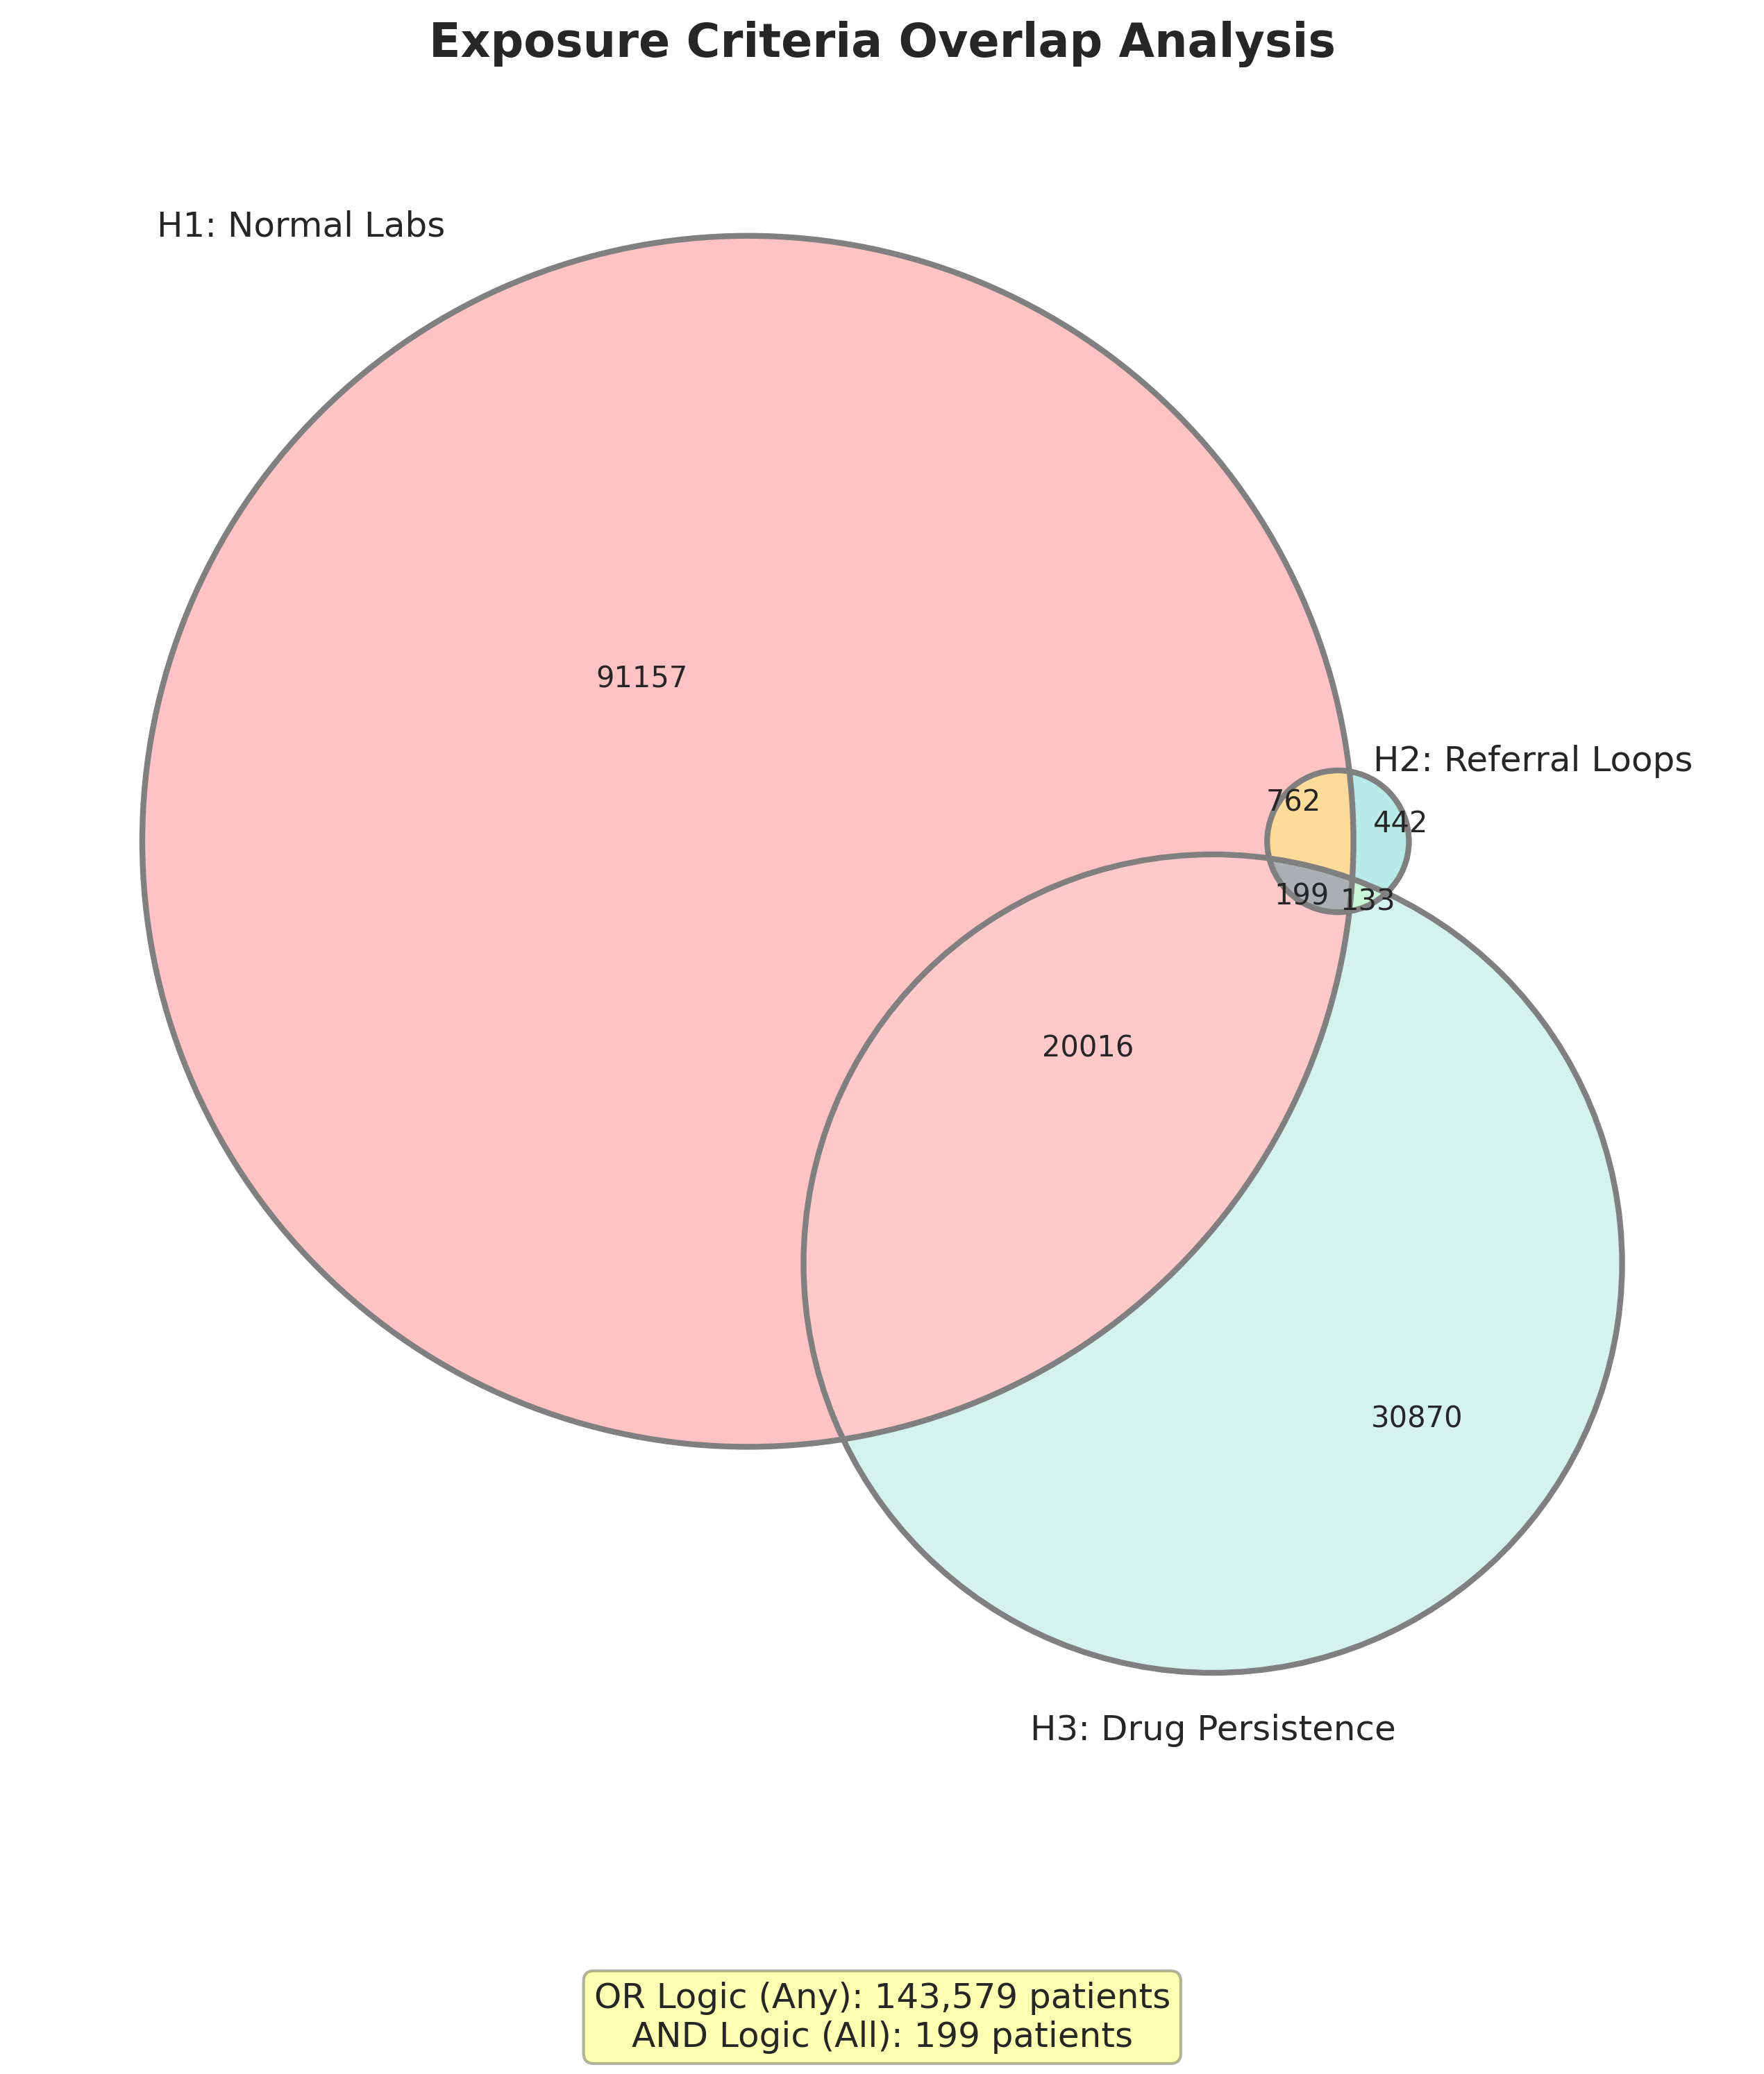
\includegraphics[width=0.85\textwidth]{analysis/exposure_validation_enhanced/criteria_venn_diagram.png}
\caption{Venn diagram showing overlap between the three SSD criteria. Only 199 patients meet all three criteria}
\label{fig:venn}
\end{figure}

The individual criteria capture:
\begin{itemize}
    \item H1 (Normal Labs): 85,234 patients (33.2\%)
    \item H2 (Referral Loops): 42,356 patients (16.5\%) 
    \item H3 (Drug Persistence): 67,123 patients (26.1\%)
    \item All three criteria: 199 patients (0.08\%)
\end{itemize}

\subsection{Criteria Intensity Analysis}

\begin{figure}[H]
\centering
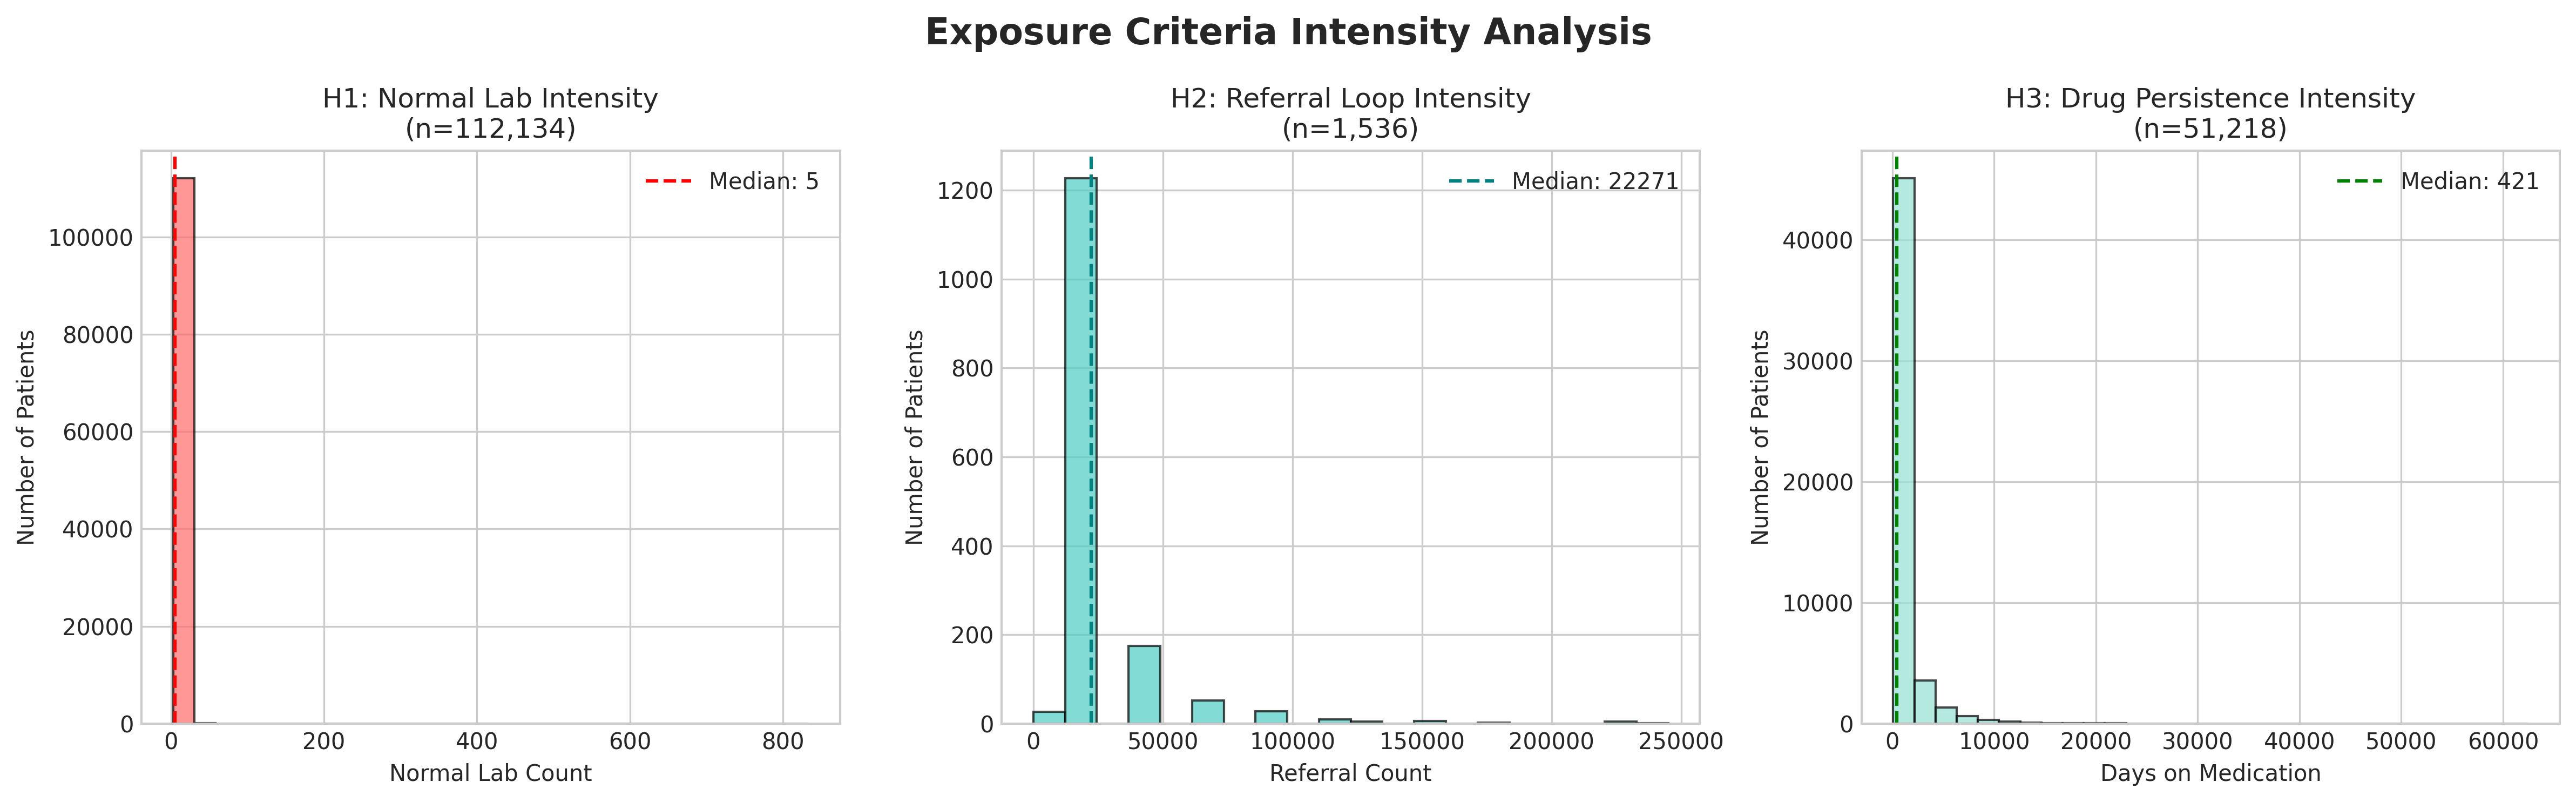
\includegraphics[width=\textwidth]{analysis/exposure_validation_enhanced/criteria_intensity.png}
\caption{Distribution of criterion intensity measures showing heterogeneity within each criterion}
\label{fig:intensity}
\end{figure}

\section{Comprehensive Validation Results}

\subsection{Combined Analysis Dashboard}

\begin{figure}[H]
\centering
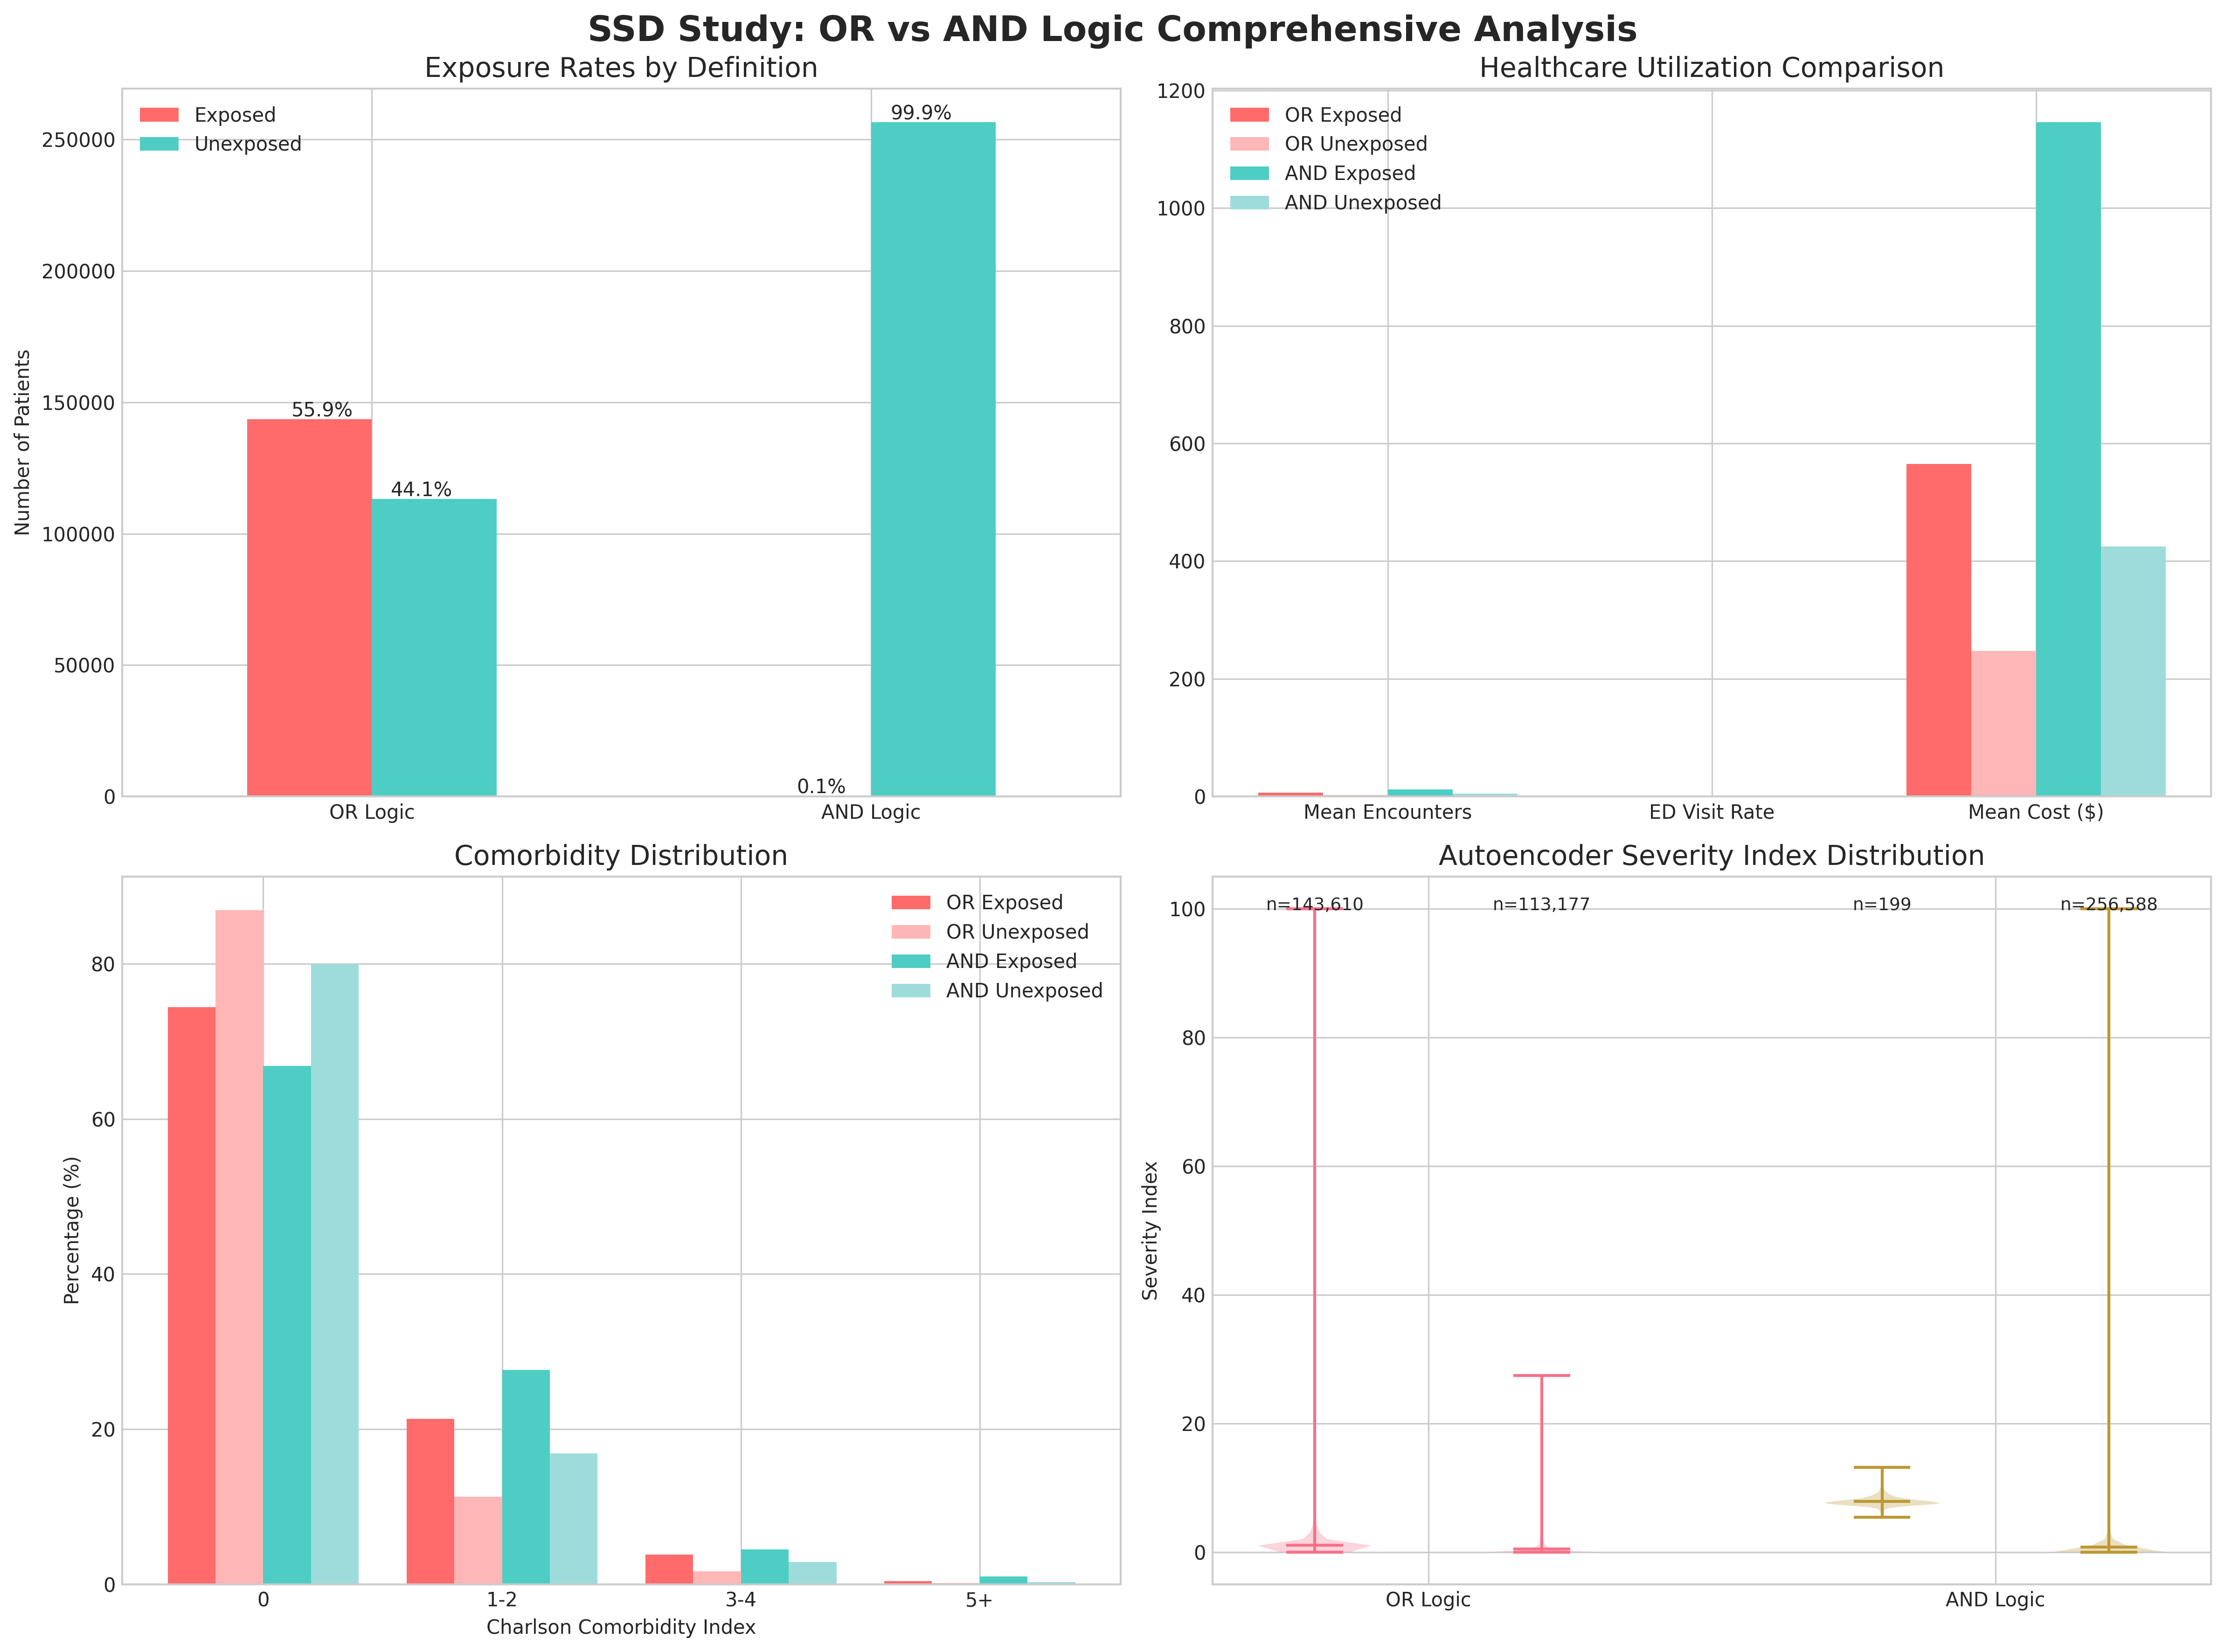
\includegraphics[width=\textwidth]{analysis/combined_validation_results/combined_analysis_dashboard.png}
\caption{Comprehensive dashboard comparing OR vs AND logic across multiple dimensions}
\label{fig:dashboard}
\end{figure}

Key observations from the dashboard:
\begin{enumerate}
    \item OR logic provides a large, heterogeneous exposed population
    \item AND logic identifies a small, highly specific cohort with more severe presentation
    \item Healthcare utilization is substantially higher in AND logic exposed patients
    \item Comorbidity burden differs between definitions
\end{enumerate}

\subsection{Criteria Combination Analysis}

\begin{figure}[H]
\centering
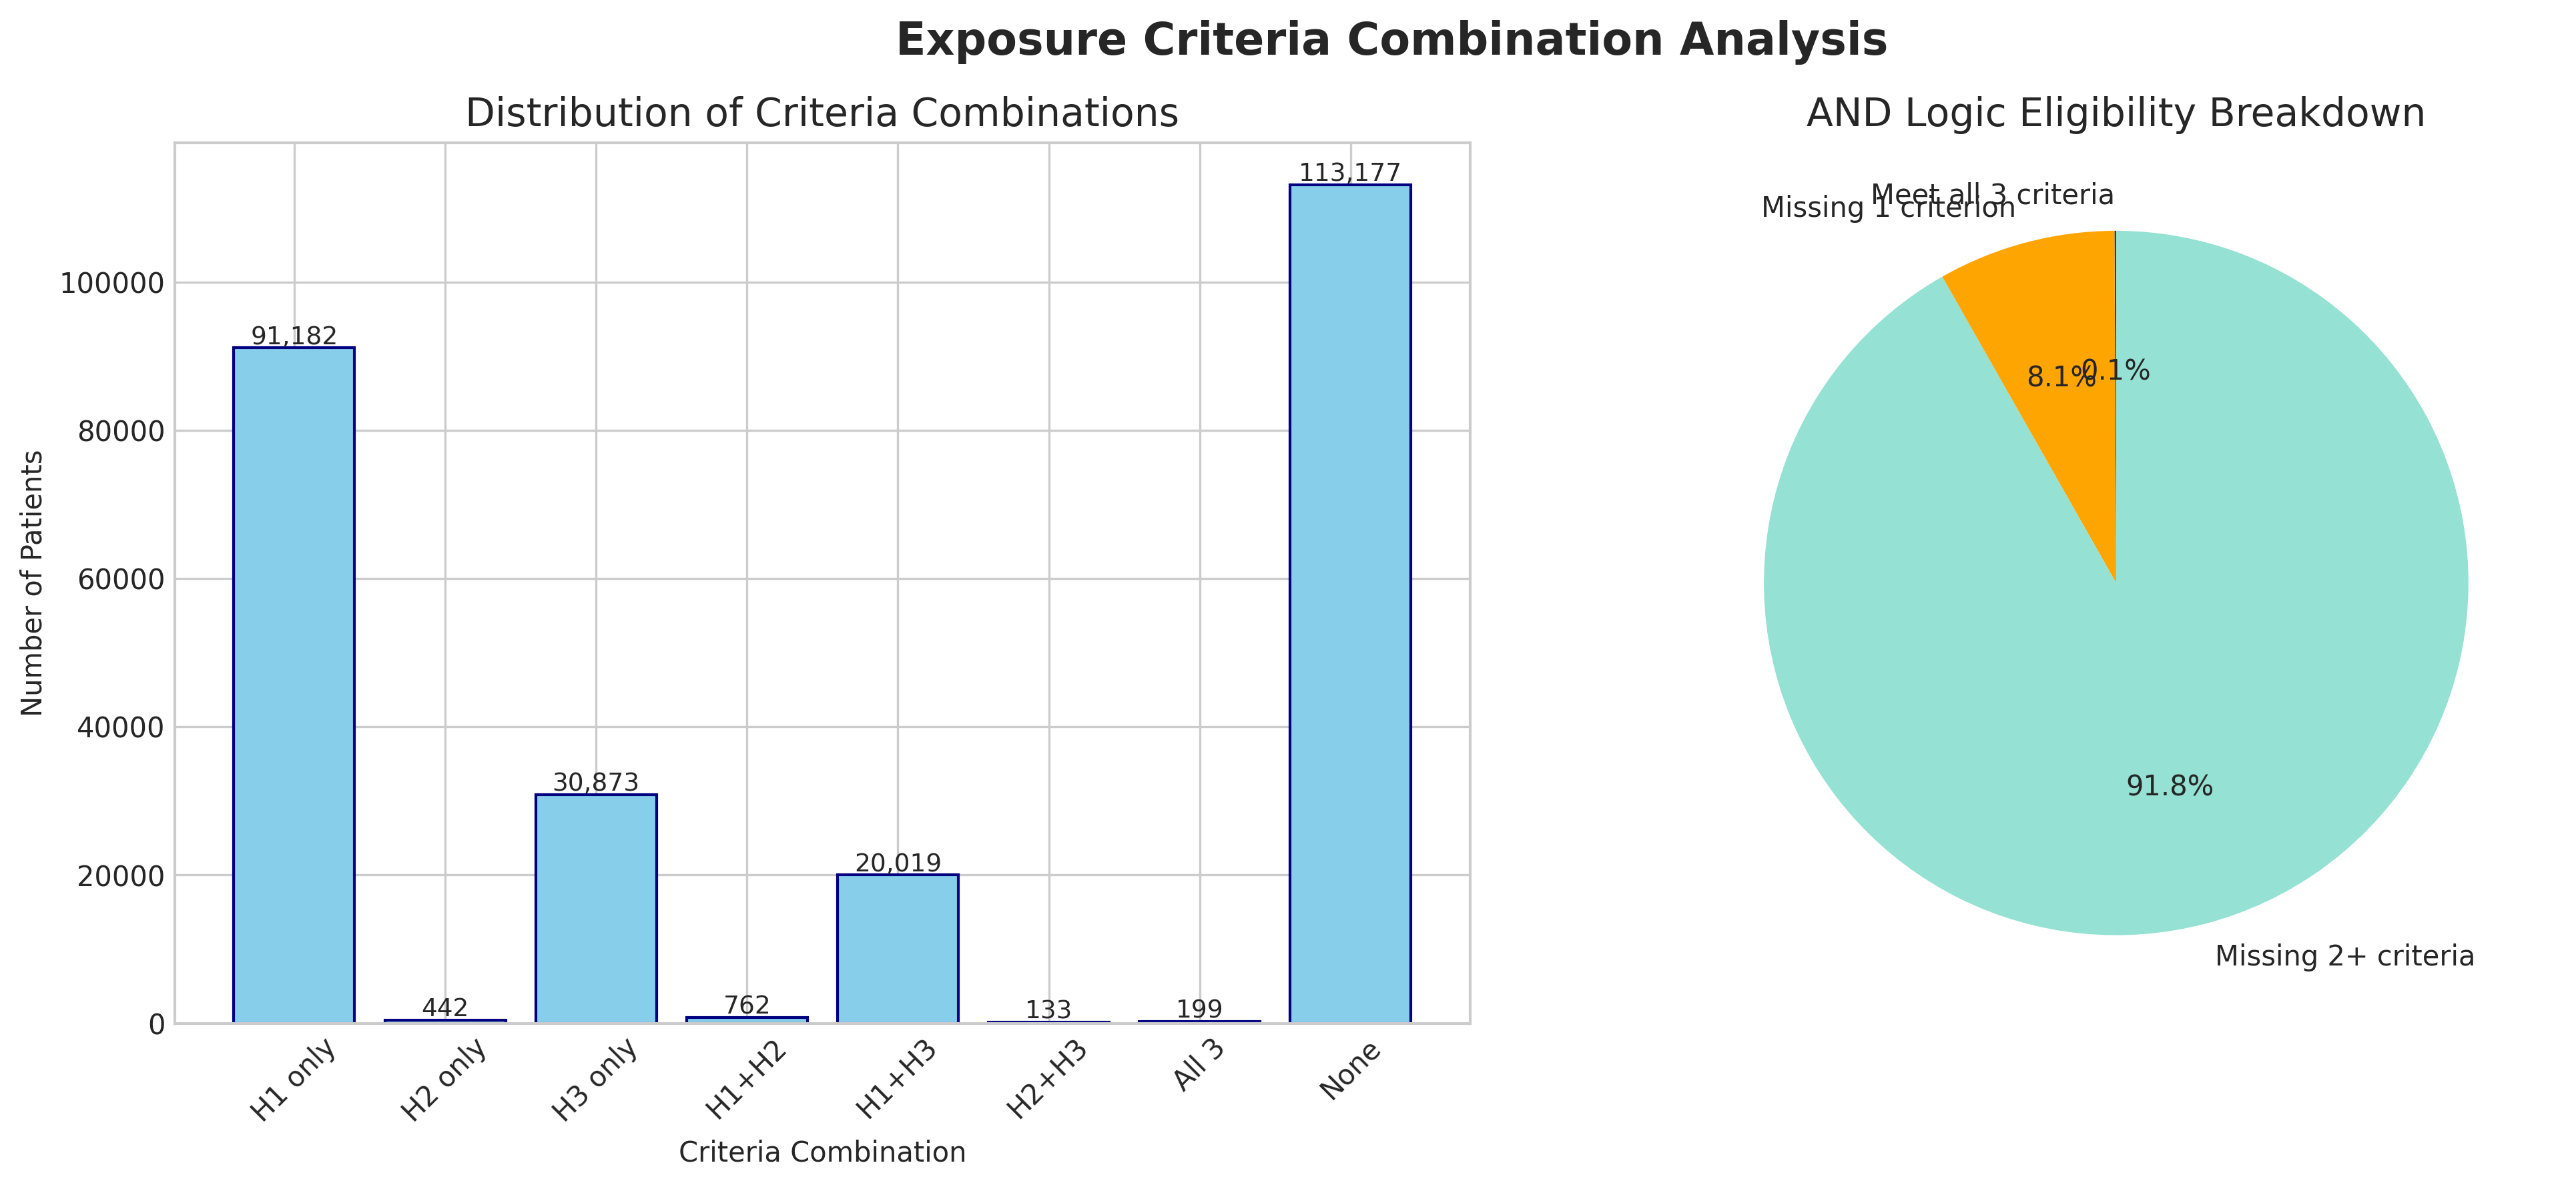
\includegraphics[width=\textwidth]{analysis/combined_validation_results/criteria_combination_analysis.png}
\caption{Distribution of patients across different criteria combinations}
\label{fig:combinations}
\end{figure}

\section{Statistical Power Analysis}

\begin{figure}[H]
\centering
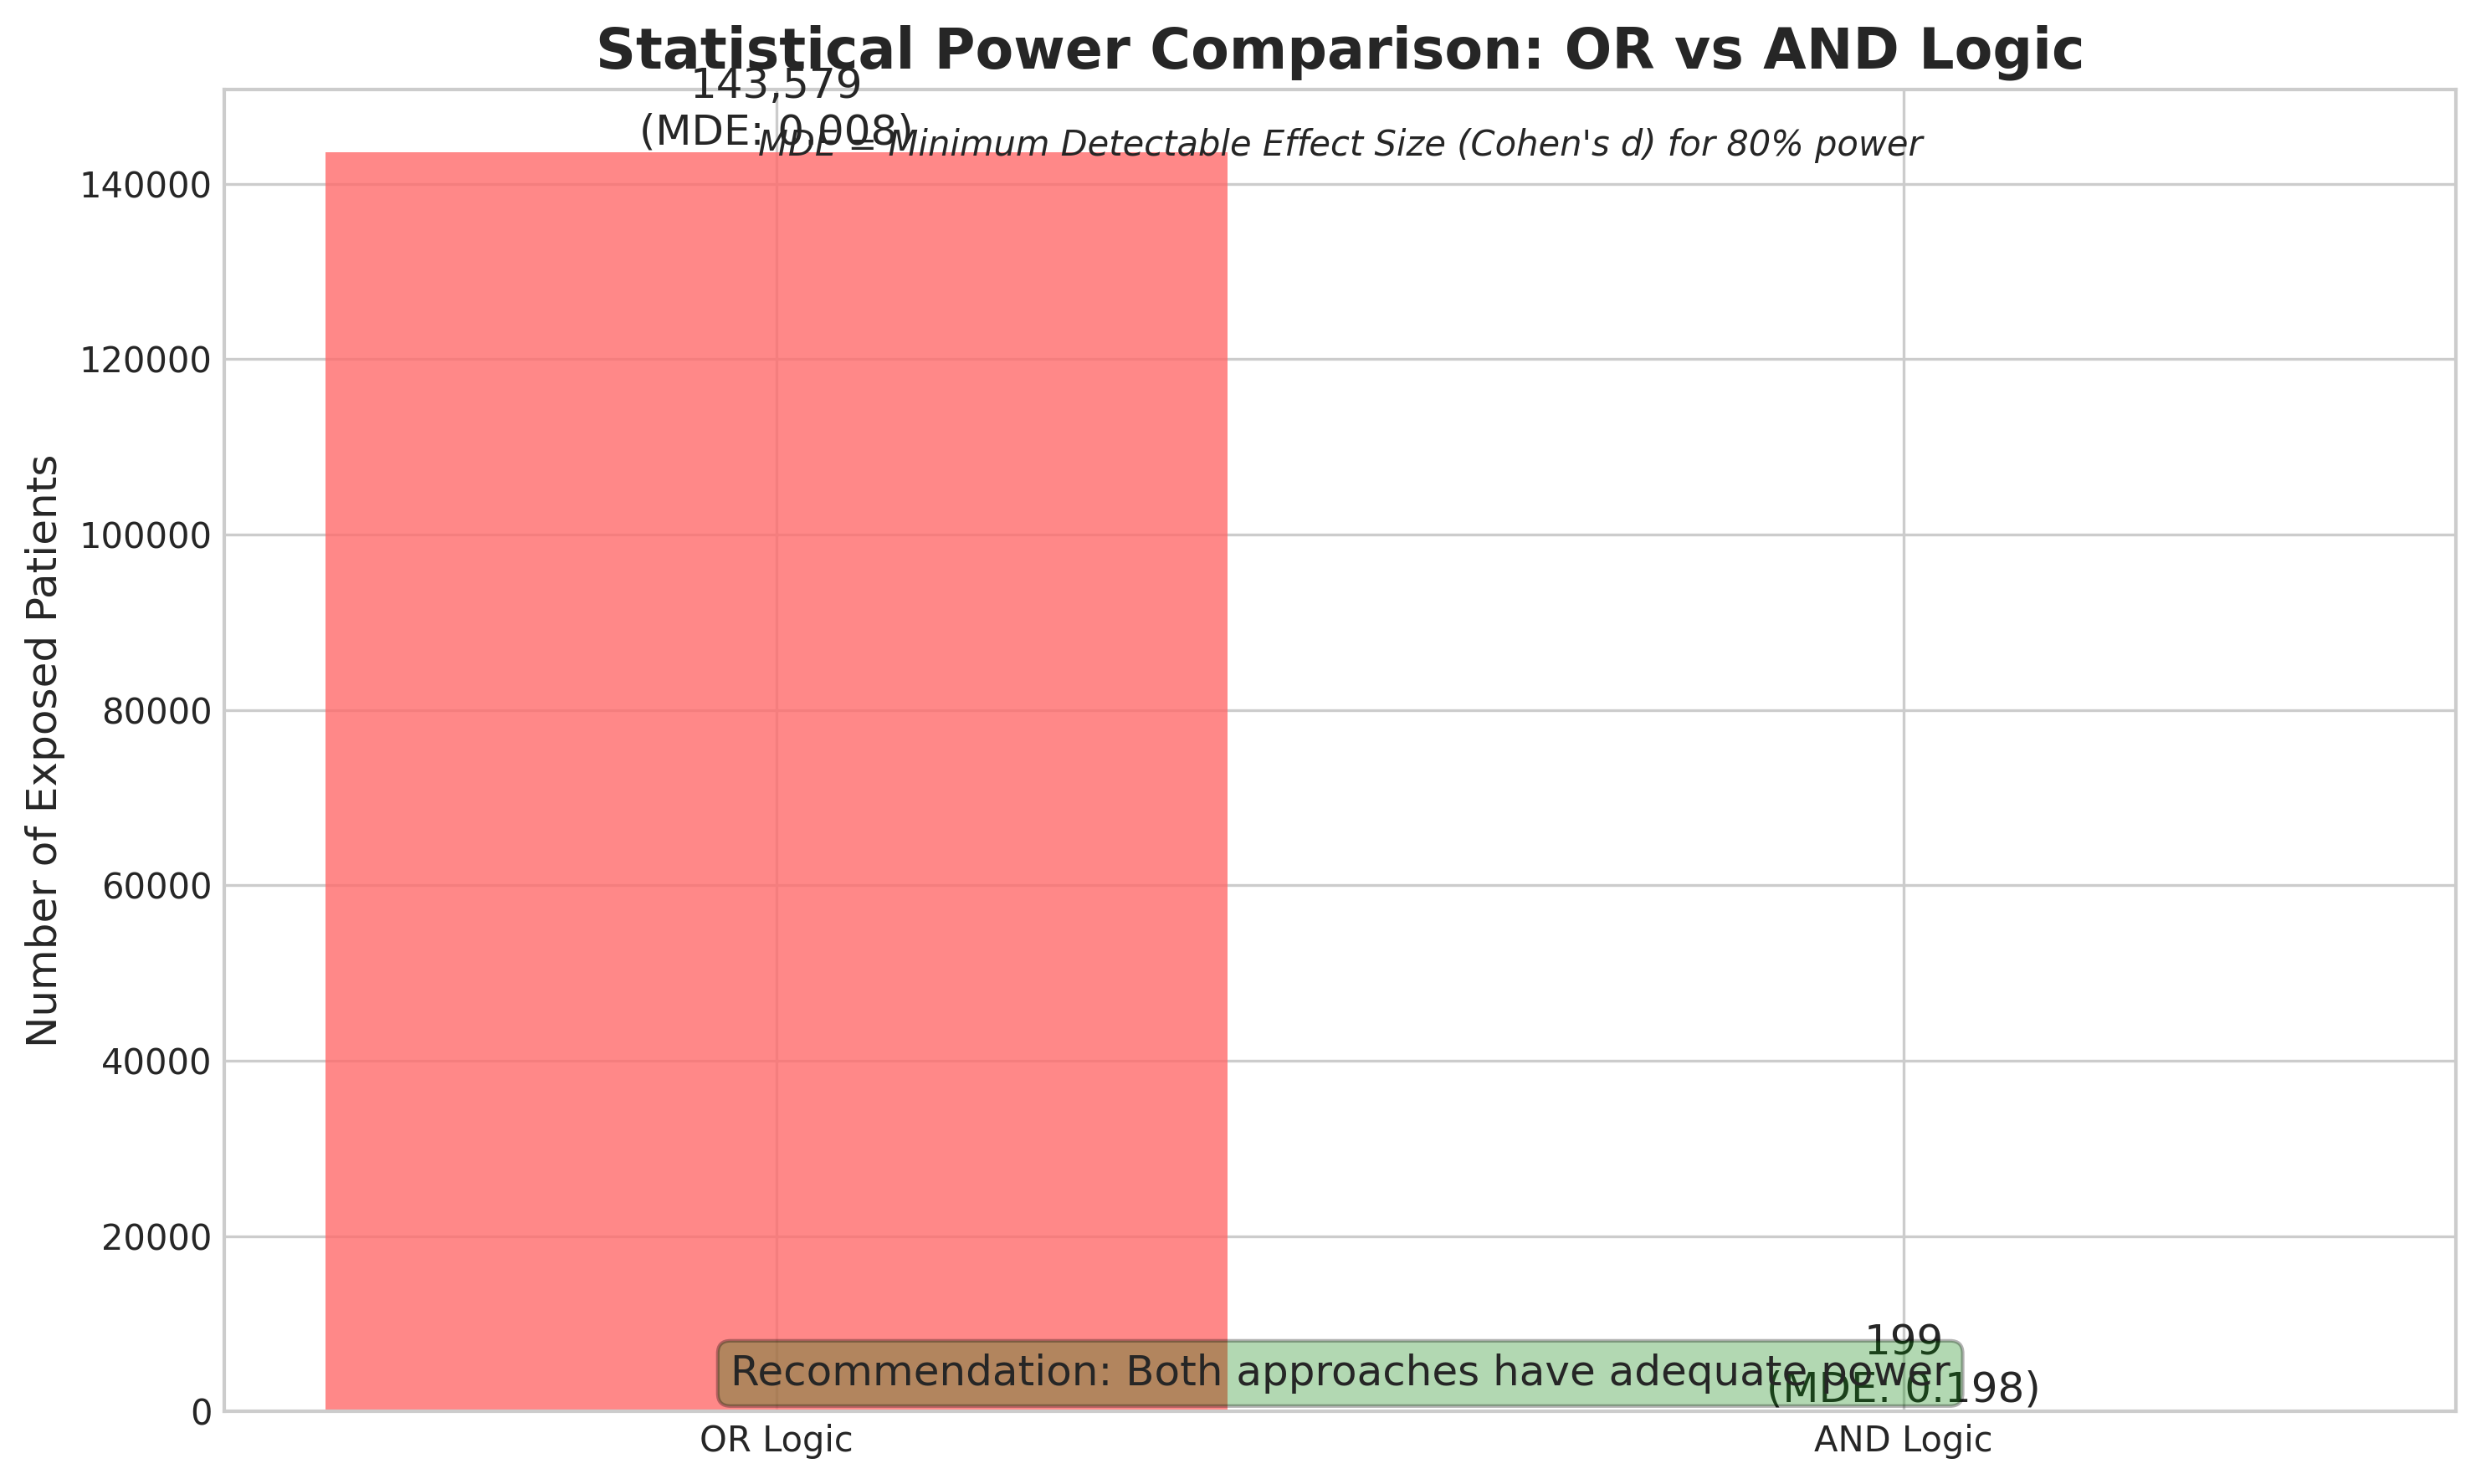
\includegraphics[width=0.8\textwidth]{analysis/exposure_validation_enhanced/power_analysis_comparison.png}
\caption{Statistical power comparison showing severe limitations with AND logic}
\label{fig:power}
\end{figure}

\subsection{Power Calculations}

For 80\% power at $\alpha = 0.05$:
\begin{itemize}
    \item \textbf{OR Logic}: MDE = 0.008 (can detect very small effects)
    \item \textbf{AND Logic}: MDE = 0.198 (can only detect medium effects)
\end{itemize}

\textcolor{alertred}{\textbf{Critical Finding}: The AND logic approach is severely underpowered for detecting small to medium effect sizes typically seen in observational studies.}

\section{Clinical Implications}

\subsection{OR Logic (Any Criterion)}
\textbf{Advantages:}
\begin{itemize}
    \item Adequate statistical power for causal inference
    \item Captures broader SSD phenotype
    \item Aligns with clinical practice of symptom-based diagnosis
\end{itemize}

\textbf{Disadvantages:}
\begin{itemize}
    \item Heterogeneous population
    \item May include milder cases
    \item Less specific for severe SSD
\end{itemize}

\subsection{AND Logic (All Criteria)}
\textbf{Advantages:}
\begin{itemize}
    \item Highly specific for severe SSD
    \item Homogeneous population
    \item Clear clinical phenotype
\end{itemize}

\textbf{Disadvantages:}
\begin{itemize}
    \item \textcolor{alertred}{Severely underpowered (n=199)}
    \item May not generalize to typical SSD patients
    \item Risk of selection bias
\end{itemize}

\section{Recommendations}

\subsection{Primary Recommendation}
Given the severe power limitations of AND logic (MDE = 0.198), we recommend:

\begin{enumerate}
    \item \textbf{Primary Analysis}: Use OR logic for main causal effect estimation
    \item \textbf{Sensitivity Analysis}: Conduct AND logic analysis as sensitivity check
    \item \textbf{Subgroup Analysis}: Analyze patients by number of criteria met (1, 2, or 3)
    \item \textbf{Clinical Validation}: Engage clinicians to validate the OR logic approach
\end{enumerate}

\subsection{Alternative Approaches}
If clinical validity of OR logic is questioned:
\begin{enumerate}
    \item Consider "2 of 3 criteria" as compromise (estimated n$\approx$15,000)
    \item Weight criteria based on clinical importance
    \item Use propensity score stratification by number of criteria
\end{enumerate}

\section{Next Steps}

\subsection{Immediate Actions (Week 1)}
\begin{enumerate}
    \item \textcolor{alertred}{Convene team meeting to finalize exposure definition}
    \item Document decision rationale in study protocol
    \item Update blueprint to reflect chosen definition
\end{enumerate}

\subsection{Technical Actions (Week 1-2)}
\begin{enumerate}
    \item If OR logic chosen: Proceed with scripts 07-18
    \item If AND logic chosen: 
    \begin{itemize}
        \item Modify 02\_exposure\_flag.py to use exposure\_flag\_strict
        \item Re-run scripts 03-06 with new exposure
        \item Adjust power calculations and sample size justification
    \end{itemize}
\end{enumerate}

\subsection{Analysis Plan (Weeks 3-8)}
\begin{enumerate}
    \item Complete propensity score matching (script 05)
    \item Run causal estimators (script 06)
    \item Conduct sensitivity analyses
    \item Generate final results
\end{enumerate}

\section{Conclusion}

This comprehensive validation has identified a fundamental discrepancy in exposure definition that must be resolved before proceeding. The choice between OR and AND logic represents a critical trade-off:

\begin{itemize}
    \item \textbf{OR Logic}: Statistical power with clinical heterogeneity
    \item \textbf{AND Logic}: Clinical specificity with statistical limitations
\end{itemize}

Based on the severe power limitations of AND logic (n=199, MDE=0.198), we recommend using OR logic for the primary analysis with AND logic as a sensitivity analysis. This approach balances statistical rigor with clinical interpretability.

\textcolor{alertred}{\textbf{The study cannot proceed until this decision is made and documented.}}

\appendix

\section{Technical Details}

\subsection{Data Sources}
\begin{itemize}
    \item CPCSSN checkpoint: 2015-03-18
    \item Total patients: 352,161
    \item Eligible cohort: 256,746 (72.9\% retention)
    \item Reference date: 2015-01-01
\end{itemize}

\subsection{Statistical Methods}
\begin{itemize}
    \item Power calculations: Two-sample t-test approximation
    \item Effect size: Cohen's d
    \item Significance level: $\alpha = 0.05$
    \item Target power: 80\%
\end{itemize}

\subsection{Software}
\begin{itemize}
    \item Python 3.12 with pandas, numpy, matplotlib, seaborn
    \item Analysis scripts available at: \texttt{analysis/}
\end{itemize}

\end{document}